\section{Routing Around Nation-States}
\label{system_design}

%The previous section showed a first step at demonstrating the extent of the 
%large-scale surveillance problem, and to our knowledge, there are no existing low-cost, 
%effective countermeasures to this problem.  As we have seen an increase in the number of 
%Internet users electing to use anonymity and circumvention systems, such as Tor, we 
%believe that there are Internet users that would also benefit from a system that 
%counters large-scale surveillance.  

From our experience conducting measurement studies of Internet paths, we have identified 
a number of obstacles standing in the way of building such systems.  These primarily include a lack 
of possible measurement methods to learn reverse paths---these are crucial because paths 
are asymmetric even at the country level---and a lack of knowledge about the locations in which 
content is replicated.  

We can surmount many of these obstacles if content providers contributed to the surveillance 
avoidance system.  To address the issue of path asymmetry, the reverse path could be measured from within the provider and used to determine if 
an unfavorable country is on the reverse path; this could be used in conjunction with our measurements 
of the forward path.  In addition, content providers could strategically publish DNS records such that when a client receives 
a DNS response, it is for a content replica that allows her to avoid a given country.  A content provider could also 
replicate content in specific regions to allow clients to access replicas without traversing a specific 
country. 

We take an approach at designing 
a system that is a first to route traffic around a given country {\it without} the help 
of providers.  Because the design does not assume any cooperation from content providers, 
the system does not (and cannot) always ensure that some Internet path avoids a 
particular country. 

{\bf Threat Model.} \system{} addresses an adversary who is restricted to a specific region of the world.  The 
adversary can be passive, and conduct surveillance, or active, and interfere with traffic. We 
realize that a country's surveillance capabilities are not limited to the infrastructure within 
its borders, but a country typically can only interfere and manipulate traffic within its borders. 
For the purposes of this system, we assume the adversary can only view and manipulate traffic 
within its borders.

An adversary who taps routers around the world, splices undersea fiber cables, or participates in 
surveillance in foreign states is out of the scope of this work; while \system{} does not address this 
type of attacker, \system{} does protect against an attacker whose interference and monitoring 
capabilities are limited to a specific land mass.

{\bf Design Goals.} Our measurement results motivate 
 the design and implementation of a relay-based avoidance system,
\system{}, with the following design goals.
\label{goals}
\begin{itemize}
\item {\bf Country Avoidance.}  The primary goal of \system{} is to
avoid a given country when accessing web content.  \system{} should
provide clients a way to route around a specified country when
accessing a domain.  This calls for the role of measurement in the
system design and systematizing the measurement methods discussed
earlier in the paper.

\item {\bf Usability.} \system{} should require as little effort as
possible from clients.  Clients should not have to download
or install software, collect any measurements, or understand how the
system works.  This requires a way for clients to automatically and
seamlessly multiplex between relays (proxies) based on different
destinations.  \system{} uses a Proxy Autoconfiguration (PAC) file to support this
function.  PAC files are supported on many types of devices, including mobile 
devices (smartphones, tablets, etc.).  Additionally, this is a mechanism that 
is already being used in systems and tools.  Many Internet users that 
use a VPN have {\it already} used a PAC file; when a user establishes a VPN connection, his 
device's proxy settings are modified to point to a PAC file.  

\item {\bf Scalability.}  This country avoidance system should be able to scale to 
many users.  Therefore, \system{} should be able to handle the addition
 of relays, as well as be cost-effective in terms of resources required. This requires 
clever measurement vantage points, such that each vantage point is representative of 
more than one client.  The PAC file allows \system{} to 
grow with the number of clients and also supports incremental deployment.

\item {\bf Non-goals.}  There are some challenges that \system{} does not
attempt to  solve; in particular, it does not provide anonymity; it routes
around  countries,
but it does not attempt to keep users anonymous in the event that traffic can
be observed.   \system{} also does not address domestic interference or surveillance. For
example, a client in the U.S. cannot use \system{} to avoid network interference 
by the United States. 
\end{itemize}


{\bf Overview.} \system{} comprises (1)~an overlay network of relays; and (2)~an oracle that
directs clients to the appropriate relays, as shown in Figure~\ref{fig:arch}.
\system{}'s relays are TCP proxy servers that allow clients to access web
content without installing custom software. \system{} uses the measurement
methods described in Section~\ref{avoid_results} to learn paths between
clients, relays, and domains; these results are stored at the oracle, which
uses the data to decide which relay a client in some location should use for
accessing a certain domain while avoiding a certain country.  The oracle
periodically computes paths for many combinations of client AS, destination,
and country.   A client can then query the oracle to determine the appropriate
relay to use to avoid a certain country en route to a particular destination.

After describing our threat model and enumerating our design goals for \system{}, we explain each component of
the system in more detail. 

%Once the TCP proxies are established, a client needs
%to learn which proxy to use when accessing a given domain.

%\begin{figure}[t]
%\centering
%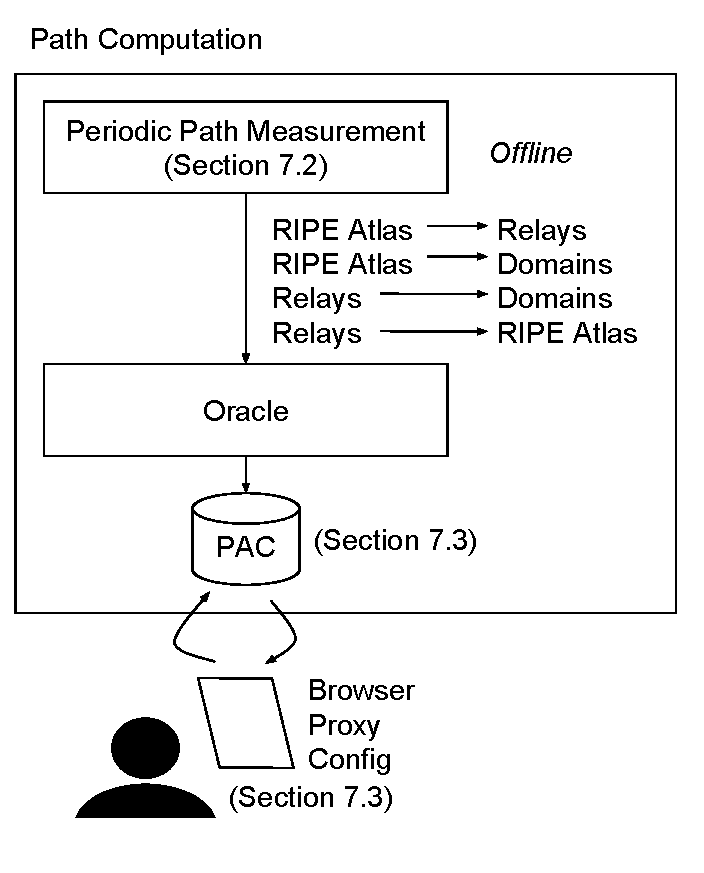
\includegraphics[width=.5\textwidth]{system_overview_updated}
%\caption{\system{} architecture. 1) Paths are computed between clients and relays, 
%relays and domains, relays and clients, and clients and domains.  2) The oracle 
%aggregates all paths.  3)  The oracle generates a PAC file that specifies which 
%domains should be accessed through which relays (based on the measured paths).  
%4) The client configures her browser to use the oracle-generated PAC file.  5) 
%The client's traffic is routed through relays (or direct paths) to access domains, 
%while avoiding a client-specified country.}
%\label{fig:arch}
%\end{figure}

\subsection{Periodic Path Measurement}

\system{} measures all paths using {\tt 
traceroute}, which is then mapped to the country level using the same methods as 
described in Section~\ref{datasets} and shown in Figure~\ref{fig:analysis_pipeline}.
The paths we measure are the: forward paths from 
the client to each relay; forward paths from each relay to each domain; forward
paths from the client to each domain; and reverse paths from each relay to the 
client. 
%Figure \ref{fig:paths} shows the forward and reverse paths when accessing 
%content using relays; the only path we cannot measure is the reverse path from 
%the domains to the relays because we have no 
%vantage point at or near the domain for running traceroute.
The portion of the reverse path from the domains to the relays is
challenging to measure due to a lack of vantage points in ASes of common
destinations. As discussed in Section \ref{pipeline}, we found that  the
forward and reverse paths are asymmetric at the country level, and therefore
\system{} cannot make any guarantees about which countries are on the path
between  domains and relays even though it has calculated the paths from
relays to domains.   Despite the lack of knowledge about this part of the
reverse path,  we can reason about possible scenarios.  If the client's
traffic is encrypted, then a country on this part of
the reverse path that the client wishes to avoid cannot perform any  traffic correlation
attacks or website
fingerprinting attacks, as the country cannot see who the client is (necessary
for website fingerprinting) and does not have access to more than one part of
the path (necessary for traffic correlation attacks).

\begin{figure}[t!]
    \centering
%    \begin{subfigure}[b]{0.4\textwidth}
        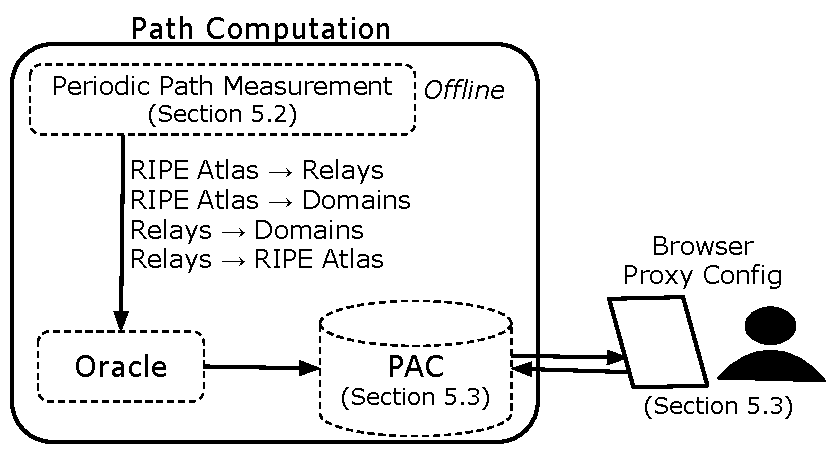
\includegraphics[width=.8\linewidth]{system_overview_updated-3}
        \caption{\system{} architecture.}
        \label{fig:arch}
%    \end{subfigure}
%    \begin{subfigure}[b]{0.4\textwidth}
%        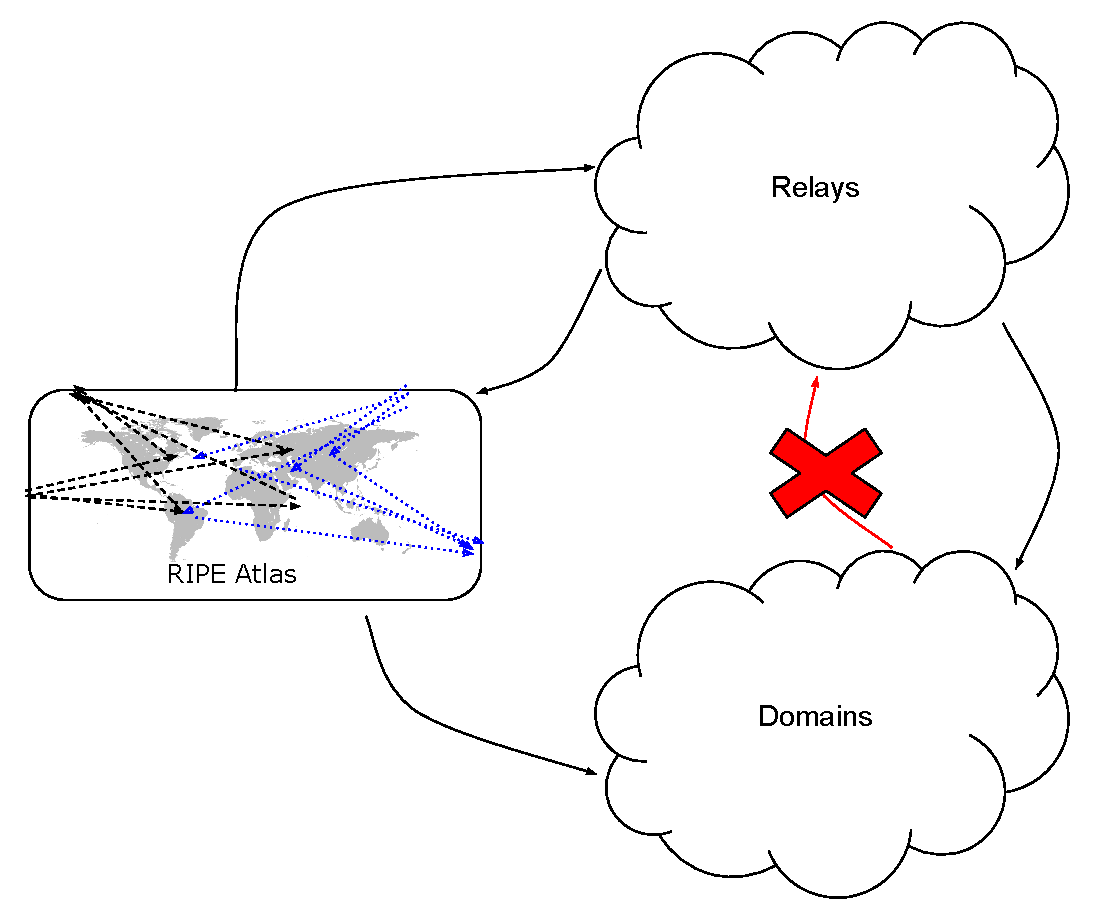
\includegraphics[width=\textwidth,height=7cm]{all_paths}
%        \caption{Paths computed in \system{}.}
%        \label{fig:paths}
%    \end{subfigure}
%    \caption{\system{} architecture, and the path
%      measurements that \system{} periodically computes.}
\end{figure}


{\bf Client-to-Relay Paths.} 
To avoid requiring the client to install custom software, \system{}
measures client-to-relay paths from RIPE Atlas probes that serve as 
vantage points for the ASes where \system{} clients might be.  \system{} selects
probes that
are geographically close the client (\eg, in the same 
country). The oracle triggers the probe to run traceroutes
to each relay.  After collecting the responses, the oracle maps 
the IP-level paths to country-level paths and stores the results.

{\bf Relay-to-Client Paths.} The \system{} relays perform
traceroutes to the IP addresses of RIPE Atlas probes, which 
represent client ASes.  They then derive country-level paths; the
oracle learns these paths from each relay.  

{\bf Relay-to-Server Paths.} Relays perform 
traceroutes to each domain.  As with paths to clients,
relays derive country-level paths and send them to the oracle.

{\bf Client-to-Server Paths.} In case a path from a client to a 
domain does not pass through the country specified to avoid {\it by default}, 
then none of the proxies should be used.  
%If a proxy is used, then it may 
%actually be causing the path to traverse more countries
%(unnecessarily).  
These paths are measured using the RIPE Atlas probes in similar
locations as the clients, and the oracle triggers traceroutes from
each of them to each of the domains.  Corresponding country-level
paths are stored at the oracle.

\system{} must recompute these paths as they change.  To our knowledge, there has not been any previous work 
on how often country-level paths change; prior work has explored how often 
AS-level paths change.  We measured the country-level paths from a RIPE Atlas probe to the 
Alexa Top 100 domains once per day for a month to see how stable country-level paths 
are.  Across the measured domains, we found the average time between path changes to 
be about five days.  Therefore, \system{} re-computes the paths every five days to incorporate the 
most recent country-level paths.  

%To measure how often country-level paths change, we 
%computed the paths from relays to domains once every two hours and once every 
%hour.  Fewer than five paths changed every two hours; the 
%results were similar for one-hour increments.  As it takes approximately 30 minutes to 
%compute all paths, \system{} re-computes the paths every one hour to incorporate 
%the most recent country-level paths.

%\begin{figure}[t]
%\centering
%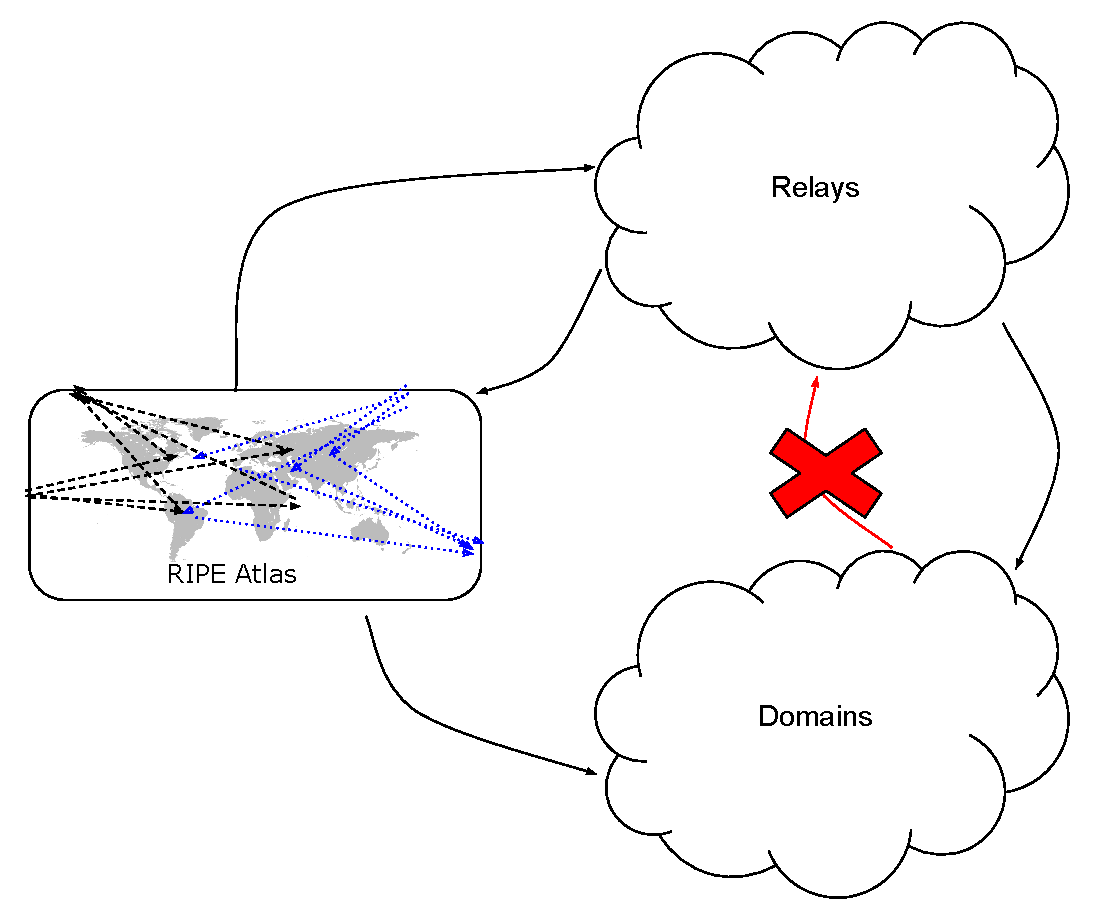
\includegraphics[width=.5\textwidth]{all_paths}
%\caption{The path of a web request through a \system{} relay, to the domain, and back. 
%1) forward path from client to relay; 2) forward path from relay to domain; 3) reverse 
%path from domain to relay; 4) reverse path from relay to client.  \system{} measures 
%all paths except for path 3) due to a lack of vantage points at domain locations.}
%\label{fig:path_components}
%\end{figure}


\subsection{PAC File Generation}
\label{multiplex}
The oracle follows four steps to decide which relay a client should
use to access a specific domain: (1)~If the default path from the
client to the domain does not pass through the specified country, then
do not use any of the relays.  (2)~Otherwise, for all the paths from
the client to the relays, select suitable relays, which are relays where the country 
to avoid is not on the forward or reverse path between the client and 
relay.  (3)~From this set, if there
is a path from a suitable relay to the domain that does not include
the specified country, then use that relay for that domain.  (4)~If
there is no path from the client through any of the relays to the
domain that does not pass through the specified country, then select
the relay that provides the most avoidance (measured by how many other
domains that avoid the specified country).
\begin{figure}[t]
\renewcommand{\lstlistingname}{Configuration}
\lstinputlisting[label={lst:pac}, language=JavaScript, frame=single,
basicstyle=\footnotesize, caption={Example PAC file.}]{example_pac.pac}
\vspace*{-0.25in}
\end{figure}
The oracle applies this decision process to each domain, which results
in a mapping of domains to relays that can be used to avoid the given
country.  To facilitate automatic multiplexing between relays,
\system{} utilizes Proxy Autoconfiguration (PAC) files, which define
how browsers should choose a proxy when fetching a URL.  In the
example PAC file in Configuration~\ref{lst:pac}, proxy 1.2.3.4:3128
should be used when accessing {\tt www.google.com}, but proxy
5.6.7.8:3128 should be used when accessing {\tt www.twitter.com}.  The
oracle uses the mapping of domains to relays to generate a PAC file,
which specifies which domains should be accessed through which proxy.
The PAC file is published online to a URL of the format
$<$client\_country$>$\_$<$country\_to\_avoid$>$\_pac.pac.  The client
uses this URL to specify their proxy configuration.  Paths are
re-computed every five days, so the contents of the PAC file are also
updated every five days.
% The PAC files are published online, which allows a client to simply
% point the proxy configuration settings to the URL that contains the
% PAC file.

\subsection{Extending \system{} with Provider Support}

While the current version of \system{} does not include support by content providers, it can be easily, incrementally,
extended to do so without any fundamental changes to the system.  This would simply require providers (or a 
CDN) to collect and share traceroute data from their server locations to different client and proxy locations; \system{} 
would then convert the traceroute data to country level paths and incorporate them into the calculation of the 
PAC files.  For content hosted in public clouds, we could set up our own VM in those same data centers and have 
\system{} collect the reverse path traceroute data to use when creating the PAC files.  

Content provider participation beyond gathering traceroute data would be even more beneficial and would lead to 
more extensive changes to \system{}.  Some of the help that content providers and CDNs could provide include 
publishing domain names that embed information about which country to avoid, strategically publish DNS records such 
that clients can take advantage of open DNS resolvers, and replicating content in diverse geographic locations.

%\section{Evaluation}
Using the \system{} implementation, we evaluate the system on it's ability to avoid a given country, performance, and scalability in terms of storage and costs.

\subsection{Country Avoidance}
As the primary goal of the system is to provide country avoidance for a given 
country, we measured how much avoidance the system achieves.  We did so by first 
calculating the number of {\it default} paths that avoid a given country.  Then 
we added a single relay, and calculated how many domains the client could 
access without traversing through the given country.  This was repeated for 
the remaining two relays.  The evaluation was conducted under the condition that 
the client wished to avoid different countries when accessing the Netherlands top 
100 domains, and the results are shown in Figure \ref{fig:avoidance_eval}.  Each 
line represents the fraction of domains accessible while avoiding the country that 
the line represents.  For example, 46\% of domains are accessible without traversing 
the United States when \system{} is not being used (0 relays), and if \system{} is 
used, then 63\% of domains are accessible with traversing the United States.

\begin{figure}[b!]
\centering
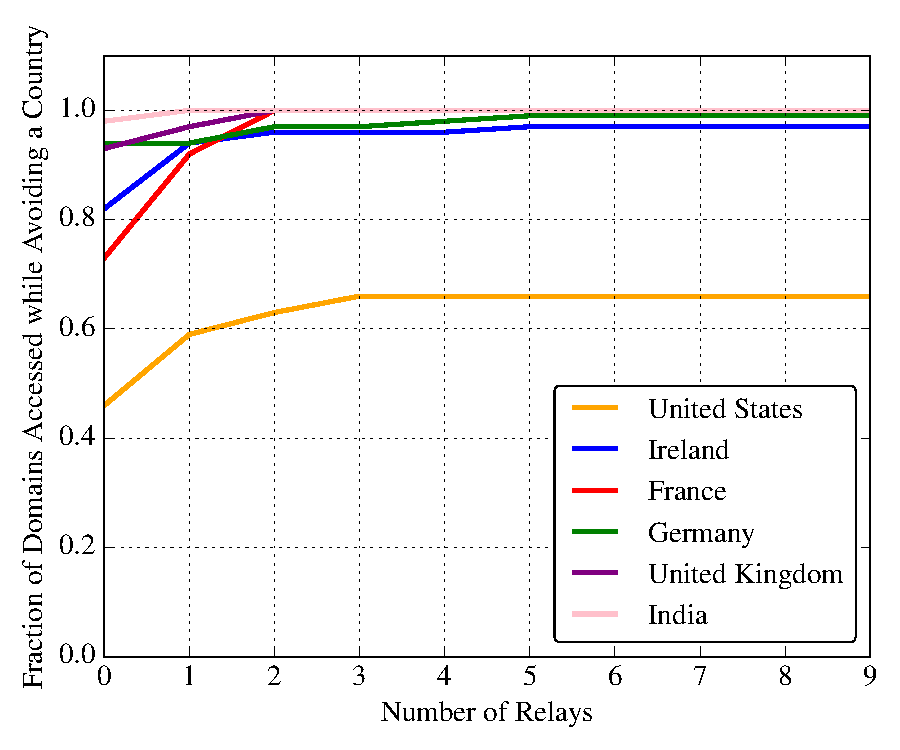
\includegraphics[width=.5\textwidth]{avoidance_n_relays}
\caption{How much avoidance different numbers and locations of relays achieve.}
\label{fig:avoidance_eval}
\end{figure}

It is evident that \system{} helps a client avoid a foreign country, as the 
fraction of domains accessible without traversing 
the specified country without \system{} is lower than with \system{}.  Additionally, 
it is clear that adding the first relay provides the greatest increase in 
provided avoidance, while subsequent relays provide a significantly 
smaller amount (or no) additional avoidance.

Figure \ref{fig:avoidance_eval} also clearly shows how much more difficult (or 
impossible) it is to avoid the United States than it is to avoid any other 
country.  Only 63\% of domains can be accessed while avoiding the United States, 
whereas almost all domains can be accessed while avoiding any other given 
country.  This confirms the results presented in Section \ref{avoid_results}, and 
emphasizes how crucial the systematization of the measurements is for enabling 
\system{}.

\subsection{Performance}
A system is not usable if the performance is significantly worse than what a user
is accustomed to.  To measure the performance of \system{}, we measure both 
the throughput and latency.

To measure throughput, we ran {\tt wget} for each 
of the top 100 domains from the client machine in the Netherlands, while 
using the PAC file.  Based on the {\tt wget} output, we calculate the number 
of seconds to access content using our system. Figure \ref{fig:latency} shows 
the CDF of the ratio of direct throughput to \system{} throughput. 

\begin{figure}[t]
\centering
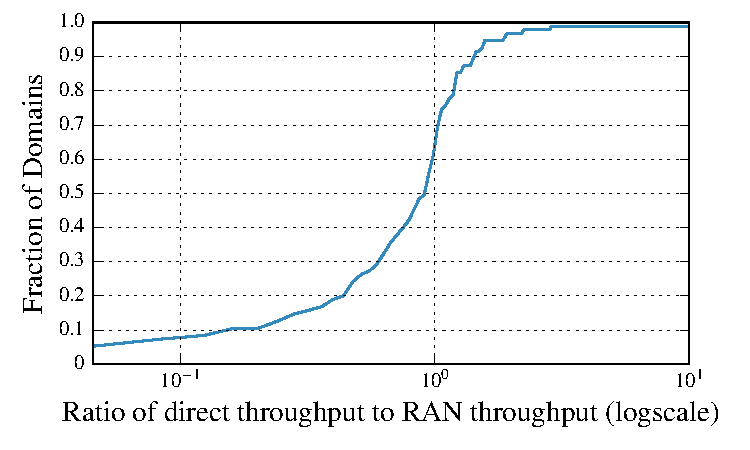
\includegraphics[width=.5\textwidth]{throughput}
\caption{Latency difference when accessing a webpage via \system{} vs. default paths. 
The difference is calculated by \system{} latency minus default latency, and represents 
the additional latency cost of our system.}
\label{fig:latency}
\end{figure}

We can see that the throughput of \system{} is not significantly worse than that 
of default paths.  In fact, in some cases the performance of \system{} is {\it 
better} than that of default paths.  This could be a result of the relays 
keeping local traffic local, or due to a closer content replica being selected. 
These results show that \system{}'s performance is comparable to the performance 
of accessing domains without \system{}.

To measure the latency of \system{}, we ran a {\tt curl} command to each of the 
top 100 domains from the client machine in the Netherlands, while using the PAC file. 
This provided the time to first byte (TTFB); we found the TTFB for both \system{} and 
direct paths, and the results are shown in Figure \ref{fig:latency}.  

\begin{figure}[t]
\centering
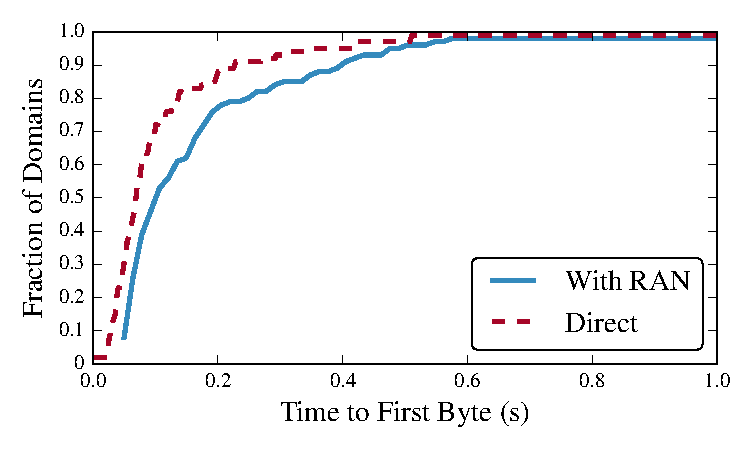
\includegraphics[width=.5\textwidth]{latency}
\caption{Latency difference when accessing a webpage via \system{} vs. default paths. 
The difference is calculated by \system{} latency minus default latency, and represents 
the additional latency cost of our system.}
\label{fig:latency}
\end{figure}

The median TTFB for direct paths is .0685, and for \system{} paths, it is .10075.  Additionally, 
the 90th percentile for direct and \system{} paths is .2253 and .40352, respectively.  This 
shows that the system's latency is greater by a factor of 2 (or 20-40ms).  \annie{Say if this is 
significant or not, especially as it relates to page load times.}

\subsection{Storage}
As the number of clients increase, and subsequently the number of paths being 
computed increases, the amount of storage must remain reasonable.  The storage 
used by paths can be calculated:

\[Storage(D,R,C) = (D x R) + 2(C x R) + (C x D) \]

D is the number of domains; R is the number of relays; C is representative of the number of 
clients.  While C {\it represents} clients, it is not the number of clients using the 
system --- it is the number of vantage points the system uses to measure paths 
from client locations.  For the prototype with a single client, the storage space for all 
paths computed is 480KB.  As there is a single PAC file for all clients in 
a country, C will grow much slower than if there was a different PAC file for 
each individual client.  There are 196 countries in the world today, and if 
paths and a PAC file were generated for each country, with 100 domains, and 
three relays, the storage would only be 94MB.  This provides plenty of storage 
for increasing the number of domains included in the PAC file or increasing 
the number of relays in the system.

\subsection{Costs}
In addition to storage, the cost of the measurements used in the system must 
be taken into account.  RIPE Atlas credits are a limited resource, and therefore 
we must earn more credits than we are spending on measurements.  The cost 
in credits follows the equation:

\[Credit\_Cost(D,R,C) = COST_{traceroute}((C x R) + (C x D))\]

Currently, the $COST_{traceroute}$ is 60, resulting in a prototype cost of 6,180 
credits, but because these paths are updated each hour, then 
the daily credit cost is 148,320 credits.  In return for hosting a RIPE Atlas 
probe, we earn 216,000 credits per day, which will support our existing 
prototype.  In order to provide for more clients, more domains, or more 
resources, we can tune the system to re-compute paths less frequently (only when necessary).

